\chapter{Act II}




\begin{figure}
   \centering
   
\includegraphics[width=.45\textwidth]{img/bg/alien.png}
   \label{fig:refinery}
\end{figure}


\begin{rpg-commentbox}{Panicking}
   
   All the firefighters take a \texttt{\textbf{STRESS}} point. Players should roleplay to how their characters react to seeing an alien for the first time. There might be a lot of questions and conversation going over the firefighters common comm channel. Eventually the fire chief will pull rank.

   \texttt{\textbf{MU/TH/UR:}} The alien in this adventure is a \texttt{\textbf{SENTRY}}.

\end{rpg-commentbox}    


\begin{rpg-commentbox}{}
   \textbf{Act 2 ends when firefighters secure the sedation ward; kill or trap the alien; or rendezvous back to the entrance.}
\end{rpg-commentbox}

\newsect




\begin{rpg-commentbox}{Everybody shut up and listen!}
   The chief explains that all that he got from his conversations with Weyland-Yutani officers is that:
   
   ``\textit{This is some very aggressive animal. Luckily, it did not escape the medical facility because of the fire containment protocols---APOLLO still has the section under lock-down and imminent detachment from the rest of the entire station. The station marshal is on his way with a small contingency force. It's surprising that they were not here already. Something is not right. Here is what we are gonna do, finish fighting the fire at the sedation ward so APOLLO considers that the facility is safe once again and then, we will think about something to take you folks out of this hell}''

   \texttt{\textbf{MU/TH/UR:}} After giving the necessary instructions, the chief states that he will speak to the marshal and see what that can do. Communication is cut loose 
\end{rpg-commentbox}



\clearpage


\section{Monster in the house}

\begin{rpg-commentbox}{Ok what we got here?}
   \texttt{\textbf{MU/TH/UR:}} Give the players some room to discuss how to proceed to the sedation ward now that they know that there is a monster lurking. The staff quarters is at least secure enough that they can have a 5 minutes (in game) conversation, but more than that and things should get back into motion, i.e., APOLLO might still detach the entire block.

   This might be very challenging in comparison with the last act where everything was clear. If players are more on the ``do objectives' side of things, you may want to use one of the firefighter NPCs or one gravely wounded mercenary to engage in the conversation add suggest alternatives. If the mercenary, let him die from their wounds after talking for a while.
\end{rpg-commentbox}




\begin{rpg-commentbox}{What do we have at our disposal?}
   \texttt{\textbf{MU/TH/UR:}} Remember players that:
   
   
   \begin{enumerate}
      \item they may have a motion tracker that can be used to track the beast. Perhaps the fire and smoke might cause interferences, but it's valid;
      \item they can probably build some molotov cocktails with the resources available at the the warehouse/pharmacy. Better burn the bitch down than be impaled alive, right?
      
      Note to \texttt{\textbf{MU/TH/UR}}, the first few times molotov is thrown at the creature, it will run away;
      
      \item There are two side pistol at their disposal;

      \item Welding torches and halligans can be used in close combat;
   \end{enumerate}

   This is challenging, but do not remove players agency, remind them of their agendas and backgrounds. Eventually, there will be a plan. Even when there is a plan, ``no plan ever survives first contact'', so it is likely that things might go off-rails. That is ok as long as everyone have fun. 
\end{rpg-commentbox}

\newsect

\begin{rpg-commentbox}{Why don't we just vent this thing?}
    Most obvious plan if players really incorporate their characters---whom have never seen an alien. Lock the beast between two corridors, set the halligans and pull the lever to vent all the air and suffocate the sucker. 
    
    This will lead to a plan following a script similar to aliens 3. The \texttt{\textbf{MOTION TRACKER}} will be extremely useful here. Use the \texttt{\textbf{STEALTH}} mode rules and ideally, let the tracker beeps guide the players to the crisis stabilization center. The area is ideal because even if a firefighter does not get to the other side of a corridor, they can trap themselves in one of the ICUs. As long as the alien is trapped, they will kill it, right?

    The plan goes sideways when they discover that the alien does not need to breath. It will start to shatter the window glass of one of the locked hatches. This can lead to a potential early death if one of the players is trapped in an ICU and the alien is in the same corridor.
\end{rpg-commentbox}


\begin{rpg-warnbox}{Death in ICU unit}
   Realizing the foolishness of their plan, a firefighter sees the alien break the ICU door and stand in front of them. Other firefighters freeze in fear. Everything happens so fast that there is barely any time to react. Even if there was, it would take time to repressurize the corridor and help their friend in peril.

   The firefighters hear the screams of pain from their companion through the open comm channel as all that they can see is the entrance of the ICU unit. Silence. A severed head flies throw zero-g, it has the eyes of someone who has seen their worst nightmares. The head flies and a trail of blood follows as black claws thunk out of the ICU corridor. Surviving firefighters retreat as the creature starts to make its escape.
\end{rpg-warnbox}
 

\newsect

\begin{rpg-commentbox}{Lock the creature in a room without any exists}
   Another option is to simply try to lock the creature in a room that has no other exits. 
   
   This is difficult because of ducts and ventilation in the facility, but might be doable in the morgue area because the morgue is where there is an incinerator and its doors are reinforced against fire/damage in case the incinerator blows. 

   Once again 
   use the \texttt{\textbf{STEALTH}} mode rules and let the firefighters make their way to the morgue.
   They can use the \texttt{\textbf{MOTION TRACKER}} to avoid the creature.

   The challenge here is how to lure the creature into the morgue main area. This is a cat and mouse game:

   \begin{enumerate}
      \item One player can make noise and probably fail stealth checks to draw the creatures attention. Whenever a player deliberately fails a roll to draw the alien, the creature moves one zone towards the players.

      \item Nearby players can keep their stealth and if there is a single player out in the open, the alien will get out of the ventilation tubes and stand tall in anticipation for the kill. A player that is face to face with the alien in this situation immediately takes \texttt{\textbf{2 STRESS}}
      and must roll for \texttt{\textbf{MANIPULATION}}. Success means slowly guiding the alien towards the morgue main door. Failure means that the alien kills the player impaling them with their tail (this is a homage to Cartwright's death).
      
     
   \end{enumerate}
   
\end{rpg-commentbox}

\clearpage

\begin{rpg-commentbox}{}
\begin{enumerate}
   \setcounter{enumi}{2}
   \item If there are multiple players in the open, and the alien is lured, it will strike from the ducts and pull one of players up. Roll a tail attack for the creature. Success means that a players starts to suffocate as the alien wraps its tail around the victims neck. Other players can try to pull the victim back to the ground with a contested \texttt{\textbf{CLOSE COMBAT}}. Failure means that the victim is dragged to the ducts out of reach from the other firefighters. The alien kills the dragged firefighter with its maw attack.

   \item If everything goes well, the remaining players must roll \texttt{\textbf{MOBILITY}} to sprint towards the creature and tackle it with \texttt{\textbf{CLOSE COMBAT}} as the player who lured the creature sprints back and pulls the hatch to seal the morgue. 
   

   \item As a final tentative to escape, the alien tail lashes towards a victim and pulls them towards the door. The hatch is closing on the person's leg and the alien starts to stand up getting ready to use its massive strength to make its way out of the room.
   
   If the players try to use all their combined strength to pull the person, the alien escapes entrapment and combat ensues. 

   If a player decides to chop the leg of person being dragged, the plan succeeds but at the cost of \texttt{\textbf{1 STRESS}} for whoever cut the leg of their friend.  \texttt{\textbf{MEDICINE}} can help stop any bleeding.     
   See \texttt{\textbf{BROKEN LEG}} rules for the injury. If assisted by another firefighter, the person who lost their leg can still move without crawling. 
\end{enumerate}
\end{rpg-commentbox}



\begin{rpg-commentbox}{Burn it in the Morgue}
   This is a variation of ``lock the creature'', but instead trying to use the morgue incinerator. The incinerator is located in one of the rooms of the morgue.
   
   On top of all the items above, the following applies.

   \begin{enumerate}
      \item When players try to start the incinerator with the creature trapped inside, the incinerator fails. The incinerator room is heavily enforced and the alien bashes several times as the players frenetically try to diagnose/reboot the incinerator panel with a \texttt{\textbf{COMM TECH}} roll. The alien will spray acid to corrode the door. This may have implications to the alien, as it losing one arm or its tail. 
      
      \item If players start the incinerator with the corroded door, it will not resist and blow. Roll   \texttt{\textbf{7 BLAST POWER}} for all. If the alien survives, it will run away.

      \item If palyers give up, they can try to sprint back to the morgue entrance with a \texttt{\textbf{MOBILITY}} roll. Go back to item 5 of ``lock the creature'' here. As the alien breaks from the incinerator room and starts pursuing the firefighters.
      
   \end{enumerate}
\end{rpg-commentbox}   

\newsect


\begin{rpg-warnbox}{Impaled}
   The firefighter who volunteered to draw the creature gazes at its polished black head. The head is so smooth and hypnotizing that they are stunned by it. The firefighter gasps for air and for courage to run away. The alien's teeth show that the creature is walking anger. As fast as lightning strikes, the creature's tail lashes upwards and impales you. It rips through your protective gear and you feel the sharp blade entering through your rectum as blood fills your mouth. 

   The alien throws the dead body in the corridor and jumps back to a duct. It could have killed everyone if it wanted to, but it is content enough seeing the firefighters' desperation.
\end{rpg-warnbox}



\begin{rpg-warnbox}{Shredded}
   Firefighters desperately tried to save you but the creature was stronger. You wished you could have passed away without air, but the creature's malice was greater almost as if it wanted to make you feel the pain about to come. The alien mouth's open, you see an inner jaw. A loud thunk sound is heard through the comm channel. A few more follow. First, it pierced through your protective helmet and took your right eye. Then, half of your left jaw. You screen in pain as the last attack rips through one of your arteries.
   
   Your blood starts to drip through the duct openings. Silence follows. Gravity makes its work and your dead body falls back as the other firefighters scream in horror.
\end{rpg-warnbox}



\begin{rpg-warnbox}{Burned}
   You and your brethren hold the door as you all pray that the incinerator reboots. Strangely, the door starts to crumble at your fingers. You swore that it was way thicker before you realize that acid is poking roles in the structure. You think that you should warn others about it. You think. The red lights flash in the celling, sirens warn that the incinerator is about to blow. You fingers feel warmer, no fire that you have ever fought is this hot. The glove's protective rubber melts and burns your hands. A loud blast erupts. Fire engulfs you and several parts of your protective gear do not resist, your body is exposed and you feel your skin boiling as more fire and shrapnel from what used to be the incinerator's door engulf you. 

   \texttt{\textbf{MU/TH/UR}} To avoid TPK, I advise that you \textbf{roll blast individually}. This may be meta, but it can also reflect that each person was in a different area of the room and the fire got to them with less or more intensity.
\end{rpg-warnbox}

\section{Sedation Ward}


\begin{rpg-commentbox}{The area}
    The sedation ward holds several hospital stretchers and a few hospital beds, all separated by curtains. A common area has some sofas and chairs for accompanying parents or family members.
    Medical equipment such as breathers, first aid kits, antibiotics and others are available in shelves on the walls. They are accessible using nurses or doctors' key cards.A huge storage container holds any hospital trash that has to be disposed at the end of a shift. 

    If the area is still on fire, the fire is mostly spreading through the curtains. Some fell from hangers and are burning on the floor. Others are still holding, but the fire makes them almost as ``firewalls''. This is a huge area divided in three zones (NE, NW, SW) and while venting it is an option the best approach is to use the fire suppression mechanism in environmental control. 

    If the fire was already suppressed, particles of halon are in the air making visibility to a bare minimum. Equipment hangs loose and other from the crackling sound of things swinging from hangers from time to time, there is a deadly silence in the air. 

    \texttt{\textbf{MU/TH/UR:}} The fire in this area started when the alien attacked and accidently tore electrical wires, which started the fire. Panic quickly ensued and a few patients and staff made to the assessment room before closing the entrance to the sedation ward. The alien killed most of the people here before the fire engulfed the area and it run away.
\end{rpg-commentbox}  


\begin{figure}[!b]
   \centering
   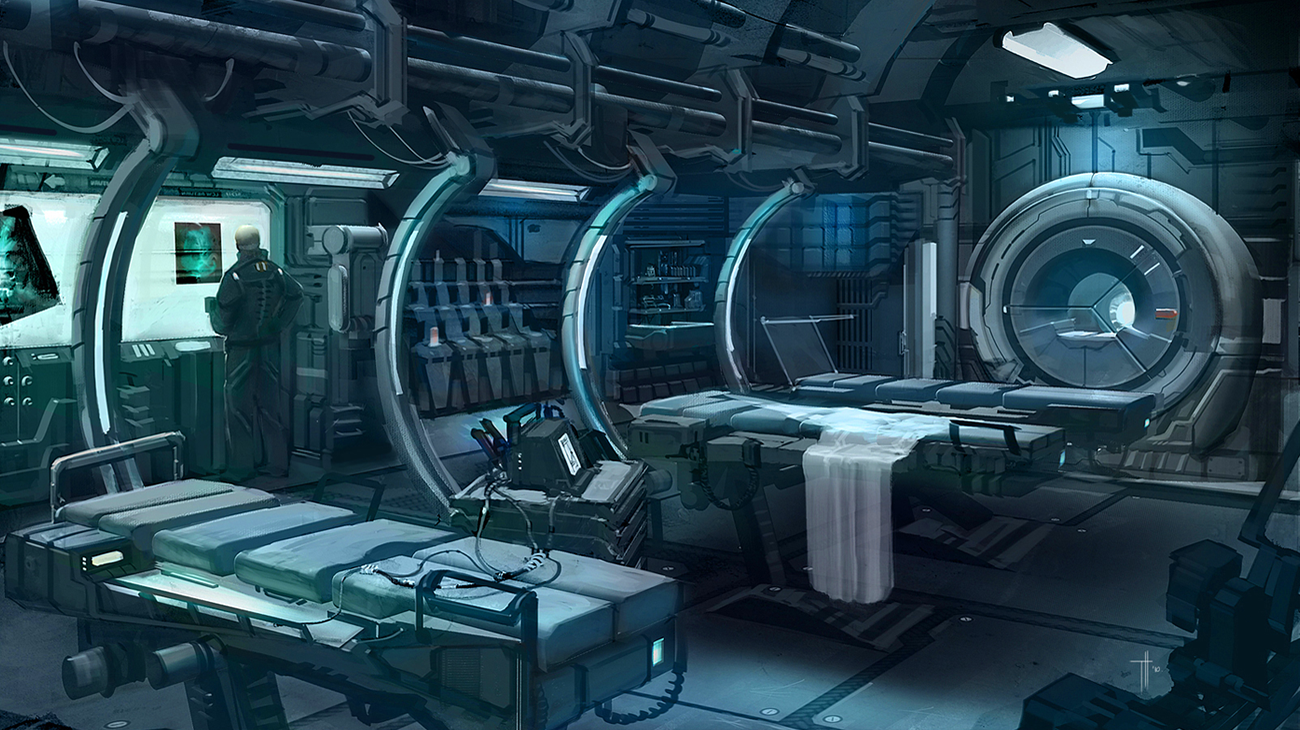
\includegraphics[width=.5\textwidth]{img/bg/medical-facility.png}
   \label{fig:refinery}
\end{figure}


\newsect

\begin{rpg-commentbox}{Clearing a path}
   Firefighters know the schematics of the building and that the fire supression mechanism is their best option. To reach environmental control, they can either go through the sedation ward or through the corridors used on their way to the VIP ICU unit. 
   
   \texttt{\textbf{MU/TH/UR:}} Remember that debris might have impeded the firefighters way, but through this side, it is possible to remove the debris (\texttt{\textbf{HEAVY MACHINERY}}) and get back to the corridor and stair cases if palyers decide to.

   \texttt{\textbf{MU/TH/UR:}} use the \texttt{\textbf{STEALTH}} mode rules and let the firefighters make their way to the sedation ward. Unless the section explicitly states that the alien appears, 
   the alien does not follow through areas with fire.
\end{rpg-commentbox}      

\newsect

\begin{rpg-commentbox}{Clearing a path - Sedation Ward}
   Firefighters must make their way through the fire spreading through the area. A \texttt{\textbf{MOBILITY}} roll allows firefighters to make their way through the zones. There can be complications moving through the area such as parts of the celling falling down (\texttt{\textbf{5 DAMAGE}}) or loose electrical wires (\texttt{\textbf{8 DAMAGE}}).

   The south-west door is also locked. Due to the damage caused by the fire, a \texttt{\textbf{HEAVY MACHINERY}} or \texttt{\textbf{COMM TECH}} at \texttt{\textbf{-3}} can open the door. Failure means that the door is half open and that the alien falls from a duct behind the players and attack the players. 
   


   \texttt{\textbf{MU/TH/UR:}} All firefighters take a \texttt{\textbf{STRESS}} point. Roll for combat. If pushed into a zone with fire, the alien will retreat. A straight \texttt{\textbf{STRENGTH}} check is required to open the door. A \texttt{\textbf{+1}}  bonus applies to every firefighter helping open the door. Using a \texttt{\textbf{spreader}} is also possible. Players can close the door behind them. The alien will back away and find another path to reach them. Remember that in the panic, some firefighters may be accidently locked on the other side with the alien.
\end{rpg-commentbox}  


\begin{rpg-warnbox}{Trapped}
   You hear screams behind you. Everyone shouts ``\textit{pull!}'' A sense of relief comes to you once you hear the pneumatic door sound. You quickly back away from the alien to find the door closed and your brethren on the other side. You bash at the door so that they can open it. You feel the cold hands of the creature tighten around your chest. Slowly its fingers poke through your protective gear and fix in your skin. The pressure is scrutiating. The creature takes pleasure as it smashes your rib cage. It could break through the ward's door, but it vanishes in the smoke.
\end{rpg-warnbox}


\clearpage

\begin{rpg-commentbox}{Environmental Control}
   Firefighters can try to manually override stuck halon ``pipes'' and suppress the fire in the sedation ward. 
   A \texttt{\textbf{OBSERVATION}} roll shows that the pipes/tubes leading to the sedation ward have been damaged but auxiliary canisters should have been fired.
   \texttt{\textbf{COMM TECH}} allows a firefighter to hack environmental control and activate the fire suppressing mechanism. 

   Firefighters can also do this manually pumping a lever. This does require  physical effort and the lever needs to be pushed thrice before it starts fire supression. Players can rotate who pushes the pump, but anyone who does it must immediately rolls for \texttt{\textbf{AIR}}. If a single player does it, that means 3 consecutive rolls.

   \texttt{\textbf{MU/TH/UR:}} If firefighters take too long here. APOLLO will start detachment procedures.
\end{rpg-commentbox} 


\section{End of Act}

\begin{rpg-commentbox}{Rendezvous at entrance}
   After all that you have been through, hearing the connecting sound of the chief's comm would be a relief. Instead, firefighters hear the voice of the station marshal.

   The marshal asks about the whereabouts of the creature. Roleplay the conversation with the firefighters. The marshal wants players to lead it to the entrance where his squad will have clear line of sight and can fusillade the creature. 

   If the alien has been dealt with, the marshal wants players to retreat to the entrance where a decontamination team will meet them and make sure that no foreign being contaminated them.  

   Throughout the conversation, firefighters also hear other people joining their comm channel. 

   \textit{--- This is bravo team. We are in position. If any big creature appears, shot it on sight! Do not take any chances, security of Anchorpoint is a priority!}

   \texttt{\textbf{MU/TH/UR:}} If players are struggling for air, give them a break. With the fire under control, APOLLO is starting to re-supply the facility. Firefighters should be able to breath without their masks. 
\end{rpg-commentbox} 

\begin{rpg-commentbox}{What happened to the chief?}
   Weyland-Yutani agents got hold of him and are making sure that he does not leak any information.

   \texttt{\textbf{MU/TH/UR:}} Let paranoia increase here. Where is the chief? What if this fire squad shot us? How can we escape?

   Raise the adrenaline, before players can come up with any clever plan, starts to narrate the steps of the alien walking through the metal panels of the facility. If the alien has been dealt with, narrate the same.

   ``\textit{Unsure whether the incoming steps are from your nemesis, you evaluate your choices: die here at the creature's hands or hope that the marshal is indeed on your side and that his team will kill the creature.}''
\end{rpg-commentbox}    